% Выбор класса документа
\documentclass[14pt]{extarticle}
% Чтобы можно было использовать русские буквы в формулах ,
%но в случае использования предупреждать об этом
\usepackage{mathtext}
\usepackage{amsfonts}
\usepackage{layout}
\usepackage[height=25cm, a4paper, hmargin={3cm,2cm}]{geometry}
% Выбор внутренней TEX−кодировки
\usepackage[TS1,T2A]{fontenc}
\usepackage [utf8x] {inputenc}
\usepackage{amssymb}
\usepackage{amsmath, amsfonts, amssymb}
\usepackage{listings}
\usepackage{color}
\usepackage{graphicx}
\usepackage{adjustbox}
\usepackage{fancyhdr}
\definecolor{bluekeywords}{rgb}{0.13,0.13,1}
\definecolor{greencomments}{rgb}{0,0.5,0}
\definecolor{redstrings}{rgb}{0.9,0,0}
\usepackage{listings}
\usepackage{afterpage}
\usepackage{tikz}
\usetikzlibrary{patterns}
\usepackage{setspace}
\onehalfspacing
\usepackage[labelsep=period]{caption}
\lstset{language=C,
showspaces=false,
showtabs=false,
breaklines=true,
showstringspaces=false,
breakatwhitespace=true,
escapeinside={(*@}{@*)},
extendedchars=\true,
inputencoding=utf8x
}
\usepackage [english , russian] {babel}
\usepackage{etoolbox}
\addto\captionsrussian{\def\contentsname{Содержание}}
\addto\captionsrussian{\def\bibname{Список литературы}}
\renewcommand{\labelitemi}{---}
\renewcommand{\thesection}{\arabic{section}.}
\renewcommand{\thesubsection}{\arabic{section}.\arabic{subsection}.}
% Начинать первый параграф раздела следует с красной строки
\usepackage {indentfirst}

% Конец преамбулы и начало текста
\begin{document}
%ТИТУЛЬНЫЙ ЛИСТ % % % % % % % % % % % % % % % % % % % % % % % % % % %
\thispagestyle{empty}
	\begin{center}
		\small
		МИНИСТЕРСТВО ОБРАЗОВАНИЯ И НАУКИ РОССИЙСКОЙ ФЕДЕРАЦИИ\\~ФГБОУ ВПО «СЫКТЫВКАРСКИЙ ГОСУДАРСТВЕННЫЙ УНИВЕРСИТЕТ ИМЕНИ ПИТИРИМА СОРОКИНА»\\
		ИНСТИТУТ ТОЧНЫХ НАУК И ИНФОРМАЦИОННЫХ ТЕХНОЛОГИЙ\\
		КАФЕДРА ПРИКЛАДНОЙ МАТЕМАТИКИ И ИНФОРМАЦИОННЫХ ТЕХНОЛОГИЙ В ОБРАЗОВАНИИ\\
	\end{center}
	\vspace{0.5cm}
	\begin{flushright}
		УТВЕРЖДАЮ\\
		Зав. кафедрой прикладной математики,\\
		к.ф.-м.н., доцент,\\
		\underline{\phantom{aaaaaaaaaaaa}}Ермоленко А. В.\\
		<<\underline{\phantom{aaaa}}>>\underline{\phantom{aaaaaaaaaaaa}} 2016г.\\
	\end{flushright}
	\begin{center}		
		\vspace{2.5cm}
		\large \textbf{ОТЧЁТ}\\
		\small об учебной практике\\
		в Сыктывкарском государственном университете\\
		в период с 27.06.2016 по 9.07.2016\\
		Тема: <<Генетические алгоритмы. Итеративный способ решения задачи раскроя>>
	\end{center}
\begin{flushright}
	\small Научный руководитель\\к.ф.-м.н., доцент:\\\underline{\phantom{aaaaaaaaaaa}}Н. О. Котелина\\
	<<\underline{\phantom{aaaa}}>>\underline{\phantom{aaaaaaaaaaa}} 2016г.\\
	\vspace{0.5cm}
	Исполнитель, студент\\145 группы:\\\underline{\phantom{aaaaaaaaaaa}}Мельников Вадим\\<<\underline{\phantom{aaaa}}>>\underline{\phantom{aaaaaaaaaaa}} 2016г.\\
\end{flushright}
\vspace{3cm}
\begin{center}
	Сыктывкар 2016
\end{center}
\newpage
%СОДРЕРЖАНИЕ % % % % % % % % % % % % % % % % % % % % % % % % % % % % % % % %
	\tableofcontents
	\thispagestyle{empty}
	\newpage
	\section{Введение}
	Экономия материала представляет собой сложную и важную проблему, с которой
	часто приходится встречаться на различных производствах, при резке различных материалов на: листы металла, стекла или дерева, трубы, профильный прокат, изделия сложной формы. Для её решения необходимо максимизировать использование материала, из которого вырезаются заготовки, что по сути и является рациональным раскроем материала. Максимизация использования материалов позволяет достичь большой экономии денежных средств.
	\paragraph{}
	На самом деле, задача раскроя является NP-полной даже для прямоугольников. Для
	фигур неправильной формы геометрическая сложность увеличивает количество совершаемых вычислений, поэтому применяются различные эвристические методы решения задачи.
	\newpage
	\section{Основные характеристика задач раскроя}
	Прежде чем приступать к рассмотрению алгоритмов решения задачи раскроя, следует рассмотреть характеристики, влияющие на то, как будет выглядеть итоговый алгоритм решения. В статье \cite{Dyckhoff} Harald Dyckhoff приводит достаточно полное описание характеристик задач раскроя.
	\subsection{Пространственные характеристики}
	Основная характеристика раскроя --- количество измерений:
	\begin{itemize}
		\item раскрой в одномерном пространстве;
		\item раскрой в двумерном пространстве;
		\item раскрой в трёхмерном пространстве.
	\end{itemize}
	\paragraph{}
	Например загрузка поддонов является задачей в двумерном пространстве. В отличие от 	задач в двух и более измерениях, задача в одномерном пространстве имеет явное решение. Достаточно подробно данная задача описывается в книге \cite{Cantorovich} Канторовича-Залгаллера --- <<Рациональный раскрой промышленных материалов>>. Так же в данной книге можно найти методы решения задач двумерного раскроя для случая прямоугольнных заготовок.
	\subsection{Количественные характеристики}
	Другая важная характеристика --- количественная. В задаче раскроя необходимо
	некоторым образом измерять количественные и качественные характеристики фигур.
	Например, площадь, длина и ширина фигур. Или количество уже расположенных фигур. Тут можно рассмотреть два варианта:
	\begin{itemize}
		\item дискретное измерение с помощью, например, натуральных и целых чисел;
		\item дробное измерение на основе вещественных чисел.
	\end{itemize}
	\paragraph{}
	Первый вариант позволяет нам подсчитывать количество изделий, уже расположенных
	на материале, а с помощью второго можно измерять различные характеристики фигур, 	такие как площадь, длина и ширина.
	\subsection{Геометрические характеристики}
	Не малую роль играют в раскрое сами фигуры, которые необходимо расположить
	на плоскости. В пространстве фигуры однозначно определяются с помощью следующих
	свойств:
	\begin{itemize}
		\item формой;
		\item размером;
		\item ориентацией;
		\item правильной или неправильной формой.
	\end{itemize}
	\subsection{Характеристики по ограничениям на результат}
	По ограничениям на результат можно выделить четыре основные группы:
	\begin{itemize}
		\item  минимальное расстояние между объектами;
		\item ориентация фигур относительно друг друга;
		\item ограничение на количество фигур;
		\item ограничение на количество совершаемых <<резов>>.
	\end{itemize}
	\paragraph{}
	Автор выделяет ещё несколько групп по различным признакам, но данные являются
	основными.
	\newpage
	\section{Постановка задачи}
	Прежде чем переходить к алгоритмам, применяемым для решения задачи раскроя, следует рассмотреть математическую постановку задачи. Задача ставится по аналогии с задачей раскроя в одномерном пространстве \cite{Nikitenkov}.
	\paragraph{}
	Имеется сырьё площади $S$, на котором неоьходимо расставить заготовки $M$ различных типов. Площади заготовок задаются вектором $s[M]$, а количество заготовок каждого типа задаётся вектором $b[M]$.
	\paragraph{}
	Пусть матрица $A[M, N]$ --- целочисленная матрица всех потенциально возможных способов раскроя одной единицы сырья, $|N|=n$ --- число таких способов. Потенциально возможный способ раскроя --- столбец матрицы $A[M, j], j\in 1:N$, удовлетворяющий условию:
	\paragraph{}
	\begin{equation}
		s[M]\cdot A[M,j]\leq S.
	\end{equation}
	\paragraph{}
	Пусть $x[M]$ --- искомый вектор, являющийся некоторым столбцом матрицы $A$. Тогда задача минимизации суммарных отходов сырья запишится следующим образом:
	\begin{equation}
		\begin{cases}
			f = S - x^T[M]\cdot s[M] \to \min \\
			x[M] \leq b[M]\\
			S - x^T[M]\cdot s[M] \geq 0 \\
			x[M] \geq 0
		\end{cases}
	\end{equation}
	\paragraph{}
	Важной особенностью задачи раскроя в двумерном пространстве является то, что не каждый столбец матрицы $A$ удовлетворяющий заданным условиям является реальным решением. Данный факт объясняется произвольностью форм заготовок, поэтому нельзя одназначно утверждать, что если заданные условия выполнены для некоторой последовательности, то эта последовательность является решением.
	\paragraph{}
	Из сказанного выше следует нелинейность задачи и то, что решение задачи может быть не только на границе многогранника, заданного условиями. Таким образом, необходимо отыскивать последовательность с помощью некоторого <<оптимизированного>> перебора. Также заданные условия никак не определяют координаты расстановки заготовок на единице сырья. Методы для решения данныъ проблем и будут описываться в дальнейшем.
	\newpage 
	\section{Генетические алгоритмы}
	Таким же образом, как нейронные сети пытаются имитировать мощь мозга, эволюционные алгоритмы (ЭА) воспроизводят биологическую эволюцию. Например, природа создала сложную структуру человеческого мозга из простейших элементов, пользуясь лишь мощью эволюции и естественного отбора. Так же как естественный отбор действует на популяции животных, позволяя лучшим выжить и передать свои гены потомкам, так же и ЭА действует, например, на последовательности раскроя, нейронные сети, электрические контуры и так далее. Они определяют качество каждого элемента в популяции, позволяя
	лучшим выжить и убивая слабейших. Далее --- очень важный шаг --- они позволяют различным решениям «скрещиваться» между собой, порождая, возможно, более жизнеспособные
	решения.
	\paragraph{}
	Генетический алгоритм (ГА) --- самый популярный из эволюционных алгоритмов. Он был изобретён Джоном Холландом в Университете Мичигана в 1975 году. По изначальной задумке, ГА использовал только бинарные числа, но для извлечения большей пользы будем пользоваться десятичными числами. Сам алгоритм состоит из нескольких частей \cite{McLeod}:
	\begin{enumerate}
		\item Кодирование проблемы в виде генов.
		\item Выведение первоначального поколения.
		\item Вычисление оценок для индивидов.
		\item Скрещивание.
		\item Мутация.
	\end{enumerate}
	\paragraph{}
	Рассмотрим ГА на применительно к задаче раскроя \cite{China}.
	\subsection{Кодирование задачи}
	Основываясь на предложенных ранее методах представления и перемещения фигур, можно заметить, что не имеет смысла включать в геном координаты положения и угол поворота так, как они будут вычислены при расположении последовательности. Достаточно кодировать лишь саму последовательность раскроя. Отметим, что для достижения результата, в геноме инидвида не должно быть повторов, соответственно каждый ген должен быть уникален. Таким образом индивидом будет являться --- последовательность просто раскроя, ведь углы постановки и координаты будут восстановлены при расположении, а геном --- порядковый номер фигуры в исходном наборе --- это позволит избежать повторов.
	\subsection{Инициализация первого поколения}
	Первое поколение индивидов оказывает огромное влияние на результат всего ГА. Чтобы получить неплохой первичный набор, можно расположить по порядку отсортированные по площади фигуры, а остальных индивидов первого поколения получить с помощью мутации.
	\subsection{Оценка индивидов}
	Оценку результата можно проводить различными способами. Можно, к примеру, ввести некоторую оценочную функцию. Рассматривая задачу раскроя, за оценку можно взять занятую фигурами площадь. Далеко необязательно использовать какой-то один фактор, например, если индивид $I$ характеризуется парой $(n, h)$, где $n$ --- число размещённых фигур, а $h$ --- высота раскроя, то можно взять за оценку данную пару. Тогда то, что индивид $I_1$ лучше, чем индивид $I_2$ можно записать через следующее отношение $\mathrm{\rho}$:
	\begin{equation}
		I_1~\rho~I_2=(n_1>n_2\lor(n_1=n_2\land h_1<h_2)).
	\end{equation}
	\paragraph{}
	Тоже самое можно записать с помощью следующей функции оценки индивидов:
	\begin{equation}
		f(I)=n+h^{-1},
	\end{equation}
	тогда достаточно сравнивать числовые значения функций. Выбранная функция будет принимать большее значение при лучшем варианте раскроя. Вообще говоря, можно использовать любую функцию, исходя из условий задачи.
	\subsection{Скрещивание}
	Рассмотрим скрещивание на следующем примере:
	\begin{enumerate}
		\item Выберем двух индивидов, например [5 2 3 7 6 1 4] и [4 6 2 1 3 5 7].
		\item Случайным образом выберем часть первого родителя, которая перейдёт в потомка: [5
		2 (3 7) 6 1 4].
		\item Удалим эти элементы из второго родителя: [4 6 2 1 (3) 5 (7)].
		\item Первого потомка получим путём копирования генов второго родителя в первого: [4 6
		3 7 2 1 5].
		\item Повторим действия 1---3, поменяв родителей местами.
		\item Второго потомка получим путём копирования генов первого родителя во второго: [5
		3 2 1 7 6 4].
	\end{enumerate}
	\paragraph{}
	Из курса математического анализа известно, что функция может иметь некоторое количество точек экстремума. Минимальное значение может достигаться в нескольких различных точках, но при этом есть и экстремумы которы минимумом не являются. 
	\paragraph{}
	В процессе скрещивания стоит использовать не только самых лучших, индивидов но и достаточно хороших в целях избежания попадания на экстремумы, не являющиеся точками минимума локальные оптимумы. Данное явление называется преждевременной сходимостью или сходимостью к квазиоптимальному решению \cite{GA}.
	\paragraph{}
	На рис. \ref{not_solve}, для некоторой функции $f:X\to Y$, продемонстрированы точки квазиоптимального и оптимального решения. На рисунке цифра 1 --- квазиоптимальное решение, а 2 --- оптимальное. 
		\begin{figure}[h]
		\begin{center}
			\begin{tikzpicture}
				\draw[->, thick] (0, 0) -- (0, 7);
				\draw[->, thick] (0, 0) -- (10, 0);
				\draw (10.3, 0) node {X};	
				\draw (0, 7.3) node {Y};	
				\draw[thick] (0.3, 7) .. controls (1.5, 3.5) .. (2, 3.5) .. controls (2.5, 3.5) .. (3.5, 4.5) .. controls (5, 6) .. (5, 6) .. controls (6, 7) .. (6.5, 3) .. controls (7, -0.5) and (8, -0.5) .. (10, 4);
				
				\draw[fill=black] (2, 3.5) circle (0.1);
				\draw[fill=black] (7.55, 0.5) circle (0.1);
				
				\draw (2, 3.8) node {1};
				\draw (7.55, 0.8) node {2};
			\end{tikzpicture}
		\end{center}
		\caption{Преждевременная сходимость}
		\label{not_solve}
	\end{figure}
	\subsection{Мутация}
	Мутация происходит после скрещивания и применяется к новым индивидам, на самом деле можно применять и к появившимся ранее. В случае раскроя в процессе мутации меняются местами два гена в последовательности. Вероятность мутации должна быть не очень высокой, приблизительно 10\%, также можно изменять экспериментально. Иногда можно переставлять не просто два гена, а целые части последовательности, но не стоит делать этого слишком часто.
	\subsection{Отбор}
	Теперь, когда для каждого индивида вычислена оценка, можно провести отбор для создания нового поколения. Самый простой вариант --- взять только те индивиды, у которых достаточно хорошая оценка. В классическом варианте генетического алгоритма, индивиды в новом поколении выбираются случайно, а вероятность попадания индивида в новое поколение будет пропорциональна его оценке. Например,
	\begin{equation}
		p_i = f_i^{-1}\sum f_k.
	\end{equation}
	\paragraph{}
	На самом деле, включать в новое поколение можно не только те индивиды, которые были выведены на данном шаге, но и те которые уже были ранее, ведь они могут быть не хуже чем те, что только что появились.
	\newpage
	\section{Заключение}
	В результате было реализовано два метода раскроя. Один на основе фигур в виде многоугольников, другой использует растровые матрицы. Первый показал свою полную несостоятельность. Он имеет огромную вычислительную сложность при очень низком качестве на реальных примерах. В дальнейшем развиваться будет только растровый метод. Он отлично подходит для фигур с большим количеством вершин и сложными формами.
	\paragraph{}
	Для наглядности результата, возьмём лист $1063\times1063$ мм. В раскройный план входят следующие наименования фигур:
	\begin{enumerate}
		\item <<Олень>> --- 5 штук, с шагом 15 градусов.
		\item <<Обезьянка>> --- 5 штук, с шагом 15 градусов.
		\item <<Голубь>> --- 5 штук, с шагом 15 градусов.
		\item <<Лошадка>> --- 5 штук, с шагом 15 градусов.
		\item <<Ангелок>> --- 5 штук, с шагом 15 градусов.
	\end{enumerate}
	\begin{figure}[h]
		\centering
		
\includegraphics[scale=0.18]{plane1}
		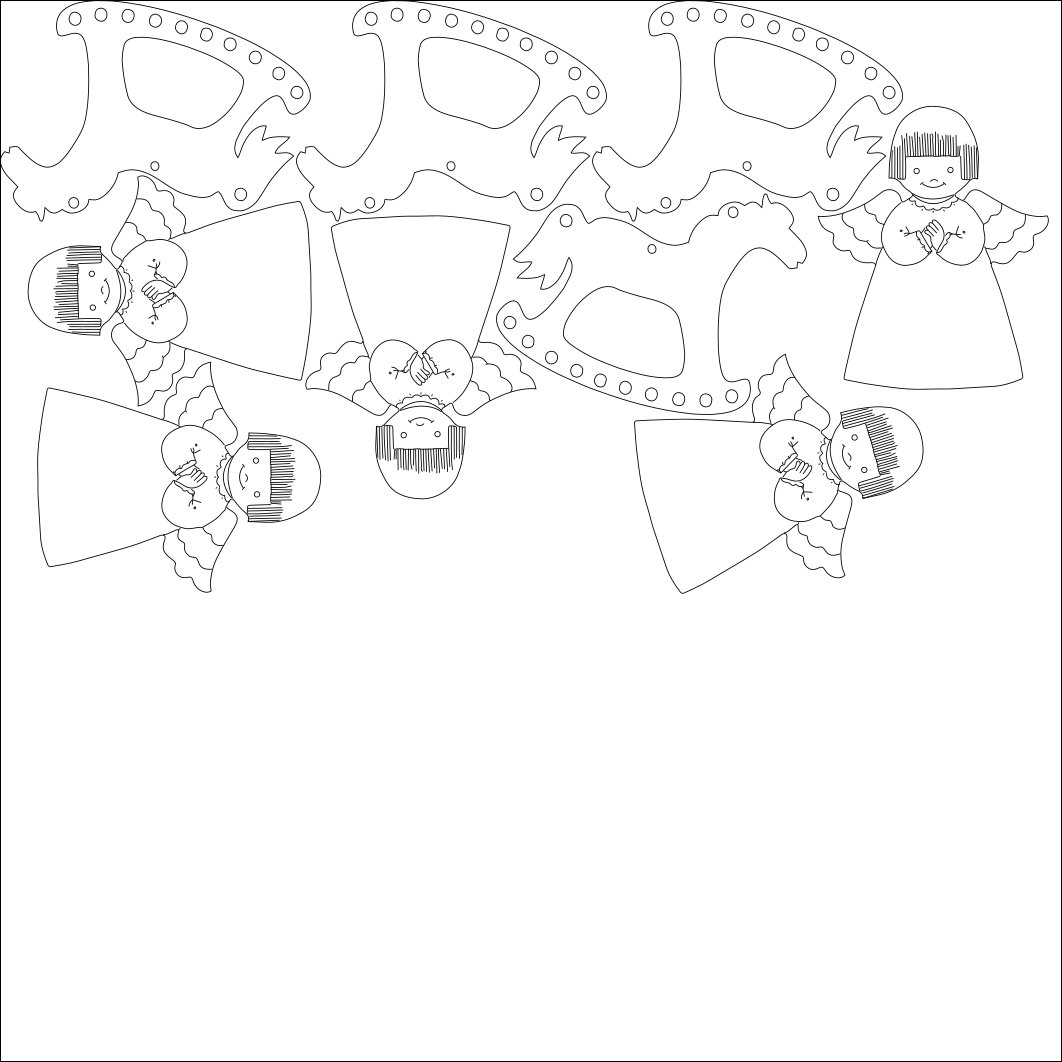
\includegraphics[scale=0.18]{plane2}
		\caption{Первый и второй раскройные листы}
		\label{plane12}
	\end{figure}
	\paragraph{}
	За $10$ итераций генетического алгоритма были достигнуты следующие результаты:
	\begin{enumerate}
		\item Раскройный план полностью выполнен с использованием двух листов.
		\item Первичная высота раскроя на первом листе --- $298.3$ мм, итоговая высота --- $292.1$ мм.
		\item Первичная высота раскроя на втором листе --- $172.2$ мм, итоговая высота --- $167.4$ мм.
	\end{enumerate}
	\paragraph{}
	Следует отметить, что для примера взят достаточно маленький лист. Экономия материала линейно возрастает с увеличением площади. Результаты можно увидеть на рис. \ref{plane12}.
	\newpage
	\section*{Приложение 1. Исходный код функций ГА}
	\addcontentsline{toc}{section}{Приложение 1. Исходный код функций ГА}
	\lstinputlisting{cmnnest.c}
	\newpage
	\begin{thebibliography}{1}
		\addcontentsline{toc}{section}{Список литературы}
		\bibitem{Dyckhoff} Dyckhoff H. A typology of cutting and packing problems // European Journal of Operational Research. № 44. 150---152 p.
		\bibitem{Cantorovich} Залгаллер В. А., Канторович Л. В. Рациональный раскрой промышленных материалов. Новосибирск: Наука, 1971.
		\bibitem{Nikitenkov} Никитенков В.Л., Холопов А.В. Задачи линейного программирования и методы их решения. Сыктывкар, 2008. 143 с.
		\bibitem{Benell_Olivera} Benell A. J., Olivera F. J. The geometry of nesting problems: A tutorial // European Journal of Operational Research. 2008. № 184. 399---402 p.
		\bibitem{McLeod} MacLeod C. An Introduction to Practical Neural Networks and Genetic Algorithms For Engineers and Scientists. 85 p.
		\bibitem{China} He Y., Liu H. Algorithm for 2D irregular-shaped nesting problem based on the NFP algorithm and lowest gravity-center principle // Journal of Zhejiang University. 2006. № 7. 571 --- 574 p.
		\bibitem{GA} Панченко Т. В. Генетические Алгоритмs; под ред. Ю. Ю. Тарасевича. Издательский дом <<Астраханский университет>>. 2007. 16 с.
	\end{thebibliography}
\end{document}